\documentclass{beamer}

\usepackage[english]{babel}
\usepackage{amssymb,amsmath,amsthm}
\usepackage{hyperref}
\usepackage{mathtools}
\usepackage{algorithm}
\usepackage{algorithmic}
\usepackage{subfigure}
\usepackage{caption}

\def\DSSC{\mathrm{Mult}\text{-}\mathrm{MSSC}}

\mode<presentation>
{
  \usetheme{Madrid}      % or try Darmstadt, Madrid, Warsaw, ...
  \usecolortheme{rose} % or try albatross, beaver, crane, ...
  \usefonttheme{structurebold}  % or try serif, structurebold, ...
  \setbeamertemplate{navigation symbols}{}
  \setbeamertemplate{caption}[numbered]
}

\title{On the Approximability of Multistage Min-Sum Set Cover}
\author{Panagiotis Kostopanagiotis}
\institute{National Technical University of Athens}
\date{16/07/2021}

\begin{document}
\bibliographystyle{plainurl}

\begin{frame}
  \titlepage
\end{frame}


\begin{frame}[plain]
	\tableofcontents
\end{frame}
%Uncomment these lines for an automatically generated outline.
\begin{frame}{Outline}
  \tableofcontents
\end{frame}

\section{Introduction}

\begin{frame}{Introduction - Static Version(MSSC)}
    \begin{itemize}
        \onslide<2-> \item Given universe $U = \{ 1, 2, ..., n \} (w.l.o.g)$
        \onslide<3 -> \item Collection $S_1, S_2, \ldots, S_m$
        \onslide<4 -> \item Select $\pi \subseteq [n!]$, Minimize: $\sum_{i=1}^m \underbrace{\pi( S_i )}_{Access Cost}$.
        \onslide<5 -> \item $\pi(S_i) = \text{The first position k s.t } \pi(k) \in S_i$.
        \onslide<6 -> \item For example: $U = \{1,2,3,4,5\}, S_1 = \{3\}, S_2=\{1,3,4\}, S_3 = \{4,5\}$
        \onslide<7 -> \item Optimal solution: \onslide<8-> $\pi = \{3,4,5,2,1\}$, \onslide<9 -> Access Cost = 1 + 1 + 2 = 4.
    \end{itemize}
\end{frame}

\begin{frame}{Motivation}
    \begin{itemize}
        \onslide<2-> \item Imagine an online store with multiple products.
        \onslide<3-> \item We have customers who have declared their interests.
        \onslide<4-> \item e.g a customer may be interested in sports and gardening, another in science, chess and videogames.
        \onslide<5-> \item We want to maintain an ordering of products, so that customers find something they like quickly.
        \onslide<6-> \item In this example $S_1, S_2, \ldots, S_m$ model the users' interests and $\pi$ is the ordering we're looking for.
    \end{itemize}
\end{frame}

\section{Previous Work}

\subsection{The Static Version of MSSC}

\begin{frame}{Min Sum Set Cover - First Results}
        \begin{itemize}
            \onslide<2-> \item Min-Sum Set Cover is NP-Hard.
            \onslide<3-> \item Greedy 4-Approximation Algorithm \cite{FLT02}.
            \onslide<4->
                \begin{block}{Greedy Algorithm for Min Sum Set Cover}\label{alg:mssc}
                    \begin{algorithmic}[1]
                        \STATE $\pi = \text{[ ]}$
                        \WHILE { $\pi$ doesn't contain all the elements of $U$}
                            \STATE Append to the end of $\pi$ the element of U that is contained in the most sets.
                        \ENDWHILE
                        \RETURN $\pi$
                    \end{algorithmic}
                \end{block}
            \onslide<5-> \item This is optimal unless P=NP \onslide<6-> (NP-Hard to approximate with factor $4-\epsilon$).
        \end{itemize}
\end{frame}

\begin{frame}{Proof Sketch}
    \begin{itemize}
        \onslide<2 -> \item Map Greedy and Optimal Solution to Histograms. 
    \end{itemize}
    \begin{figure}
            \centering
            \onslide<3 ->
                \begin{subfigure}
                  \centering
                  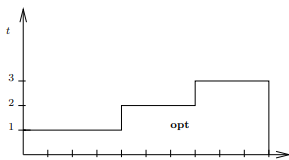
\includegraphics[width=.4\linewidth]{histogram_opt.png}
                  \label{fig:sub1}
                \end{subfigure}%
            \onslide<4 ->
                \begin{subfigure}
                  \centering
                  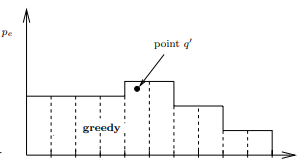
\includegraphics[width=.4\linewidth]{histogram_greedy.png}
                  \label{fig:sub2}
                \end{subfigure}%
            \label{fig:histograms}
        \end{figure}
    \begin{itemize}
        \onslide<5-> \item Shrink Greedy vertically and horizontally by 2. 
    \end{itemize}
        \onslide<6-> \begin{figure}
            \centering
            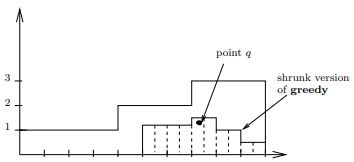
\includegraphics[width=.6\linewidth]{histogram_fit.png}
            \label{fig:my_label}
        \end{figure}
\end{frame}

\subsection{The generalized Version}

\begin{frame}{Generalized MSSC}
    \begin{itemize}
        \onslide<2-> \item What if the customers are demanding?
        \onslide<3-> \item Along with $S_1, \ldots, S_m$ we are given: $K(S_i) \leq |S_i|$.
        \onslide<4-> \item Find $\pi$ to minimize: $\sum_{i=1}^m \pi_{K(S_i)} (S_i)$.
        \onslide<5-> \item Here $\pi_{K(S_i)} (S_i) = \text{the position of the } K(S_i) \text{-th element of } S_i \text{ in } \pi$.
        \onslide<6-> \item Firstly introduced in \cite{AGY09} by Azar et. al. $O(logn)$-apx.
        \onslide<7-> \item Constant factor approximation in \cite{BGK10} by Bansal et al. 485-apx.
        \onslide<8-> \item LP-Rounding Approach, Skutella and Williamson \cite{SW11} improve it to 28-apx.
    \end{itemize}    
\end{frame}

\begin{frame}{GMSSC - Fractional LP}
    \begin{equation*}
        \begin{array}{ll@{}ll}
            \text min & \displaystyle \sum_{t = 1}^n \sum_{i = 1}^{m} ( 1 - y_{i,t} ) &\\
            \text{ s.t } & \displaystyle \sum_{e \in U} x_{e,t} = 1~~~~\text{ for all }t \leq n &&\\
            & \displaystyle \sum_{t=1}^{n} x_{e,t} = 1~~~~\text{for all }e \in U &&\\
            & \displaystyle \sum_{e \in S \setminus A} \sum_{t'<t} x_{e,t} \geq (K(S_i) - |A|) \cdot y_{i,t}~~~~\text{ for all } i \leq m, A \subseteq S_i, t \leq n &&\\
            & \displaystyle x_{e,t}, y_{i,t} \in [ 0, 1 ] ~~~~\text{ for all } e \in U, i \leq m, t \leq n
        \end{array}
    \end{equation*}
    \onslide<2-> Use $x_{e,t}$ to order the elements and construct $\pi$.
\end{frame}

\begin{frame}{GMSSC - Randomized Rounding}
    \begin{figure}
        \onslide<2-> 
            \begin{subfigure}
                \centering
                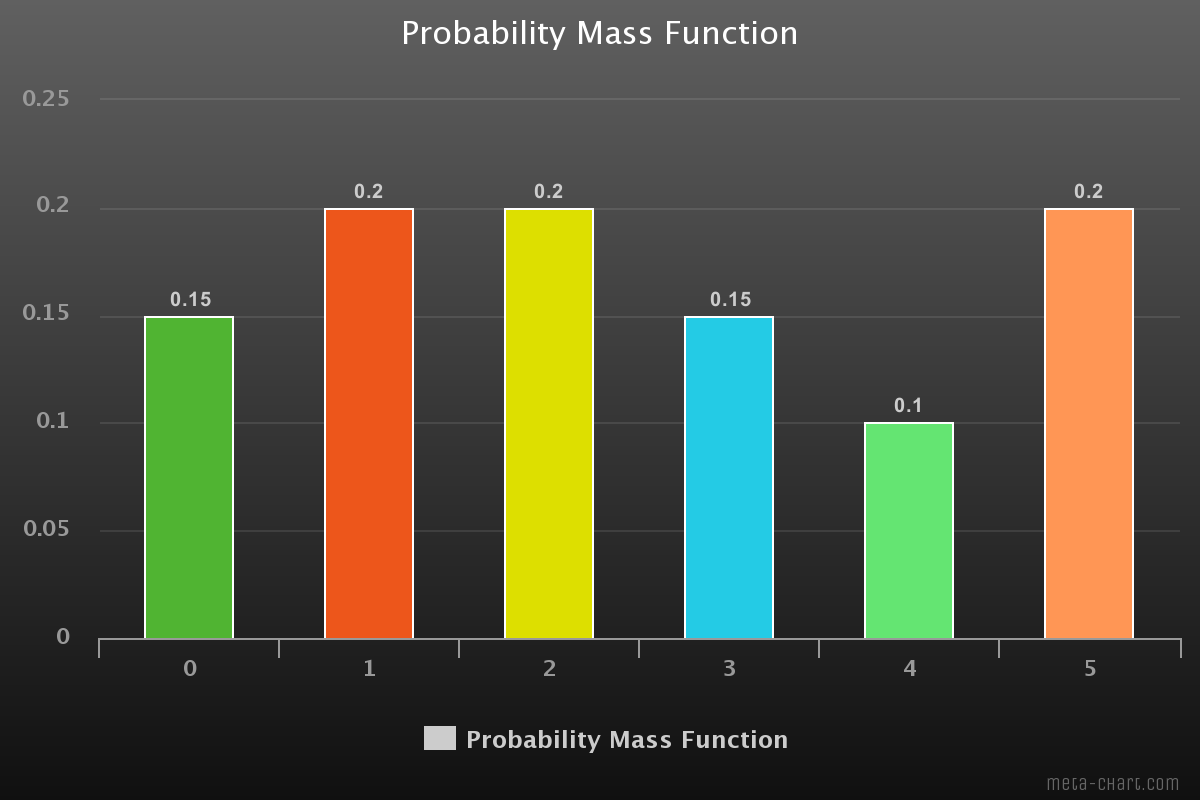
\includegraphics[width=0.4\linewidth]{prob_mass.png}
                \label{fig:prob_mass}
            \end{subfigure}
        \onslide<3->
            \begin{subfigure}
                \centering
                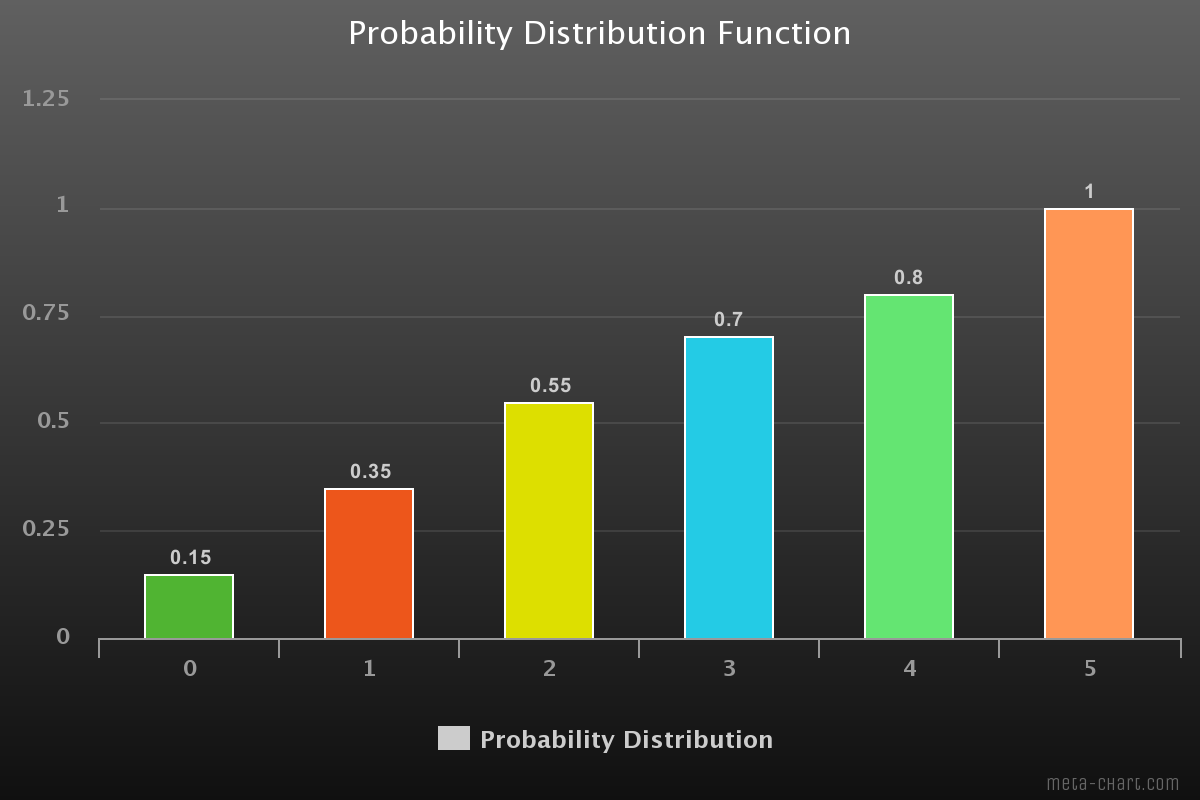
\includegraphics[width=0.4\linewidth]{prob_dist.png}
                \label{fig:prob_dist}
            \end{subfigure}
    \end{figure}
    
    \onslide<4-> Pick uniformly at random $\alpha \in [0,1]$.
    
    \begin{figure}
        \onslide<5->
            \begin{subfigure}
                \centering
                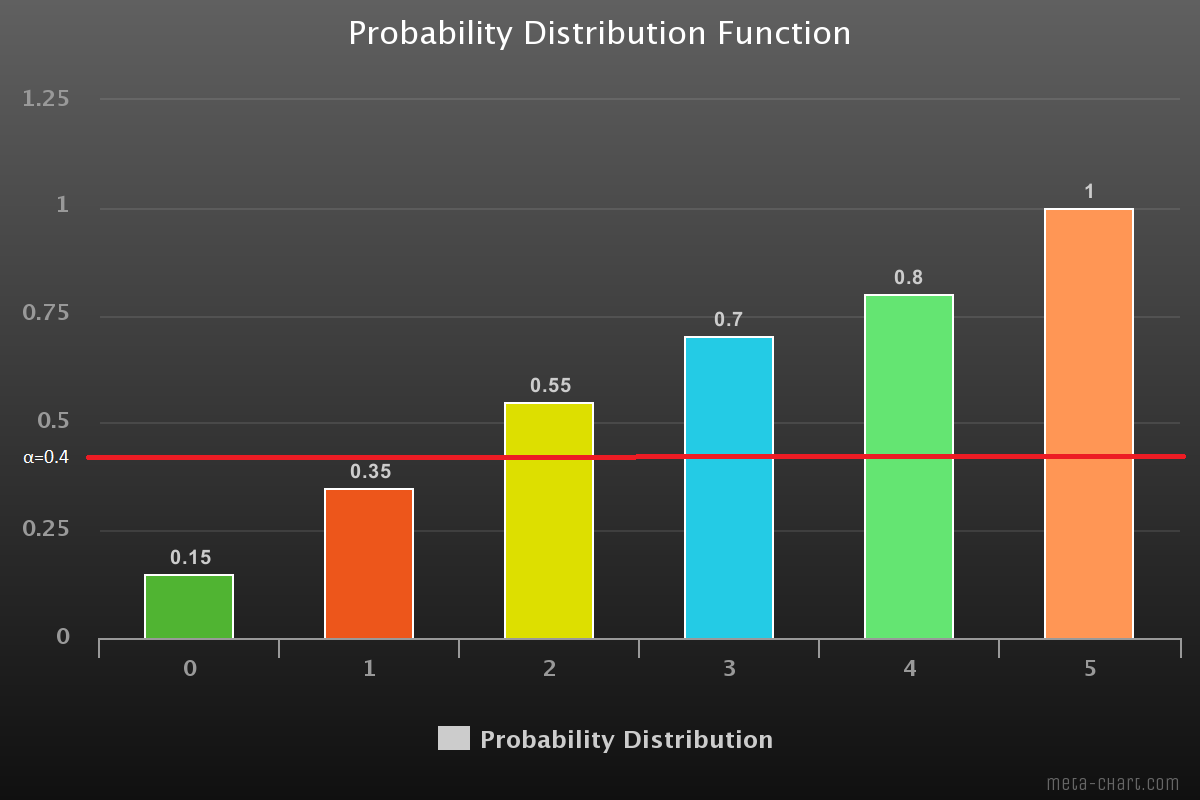
\includegraphics[width=0.4\linewidth]{pick_a.png}
                \label{fig:horizontal_line}
            \end{subfigure}
        \onslide<6->
            \begin{subfigure}
                \centering
                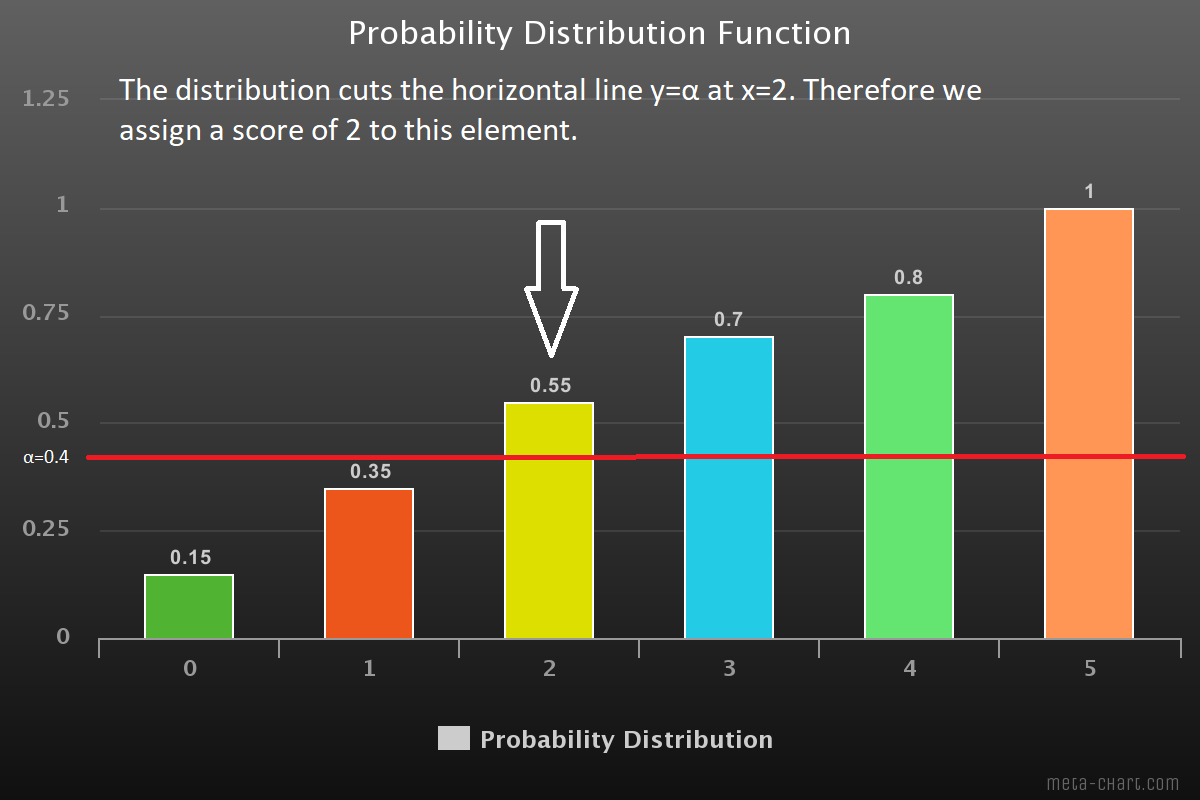
\includegraphics[width=0.4\linewidth]{pick_a_explain.png}
                \label{fig:ranking}
            \end{subfigure}
    \end{figure}
    
    \onslide<7-> Sort in order of non-decreasing score.
\end{frame}

\subsection{The Online Version of MSSC}

\begin{frame}{Multistage Min-Sum Set Cover}
    \begin{itemize}
        \onslide<2-> \item What if users' interests change over time?
        \onslide<3-> \item Given $S_1, S_2, \ldots, S_T \subseteq\{1,2,\ldots,n\}$, construct sequence of permutations $\pi^1, \pi^2, ..., \pi^T$
    \end{itemize}
    
    \onslide<4-> $$\text{Minimize} \underbrace{\sum_{t=1}^T \pi^t ( S_t )}_{\text{Access Cost}} + \underbrace{\sum_{t=1}^T \#inversions( \pi^t, \pi^{t-1} )}_{\text{Moving Cost}}$$
    
    \begin{itemize}
        \onslide<5-> \item W.L.O.G $\pi^0 = [ 1,2, \ldots, n ]$.
    \end{itemize}
\end{frame}

\begin{frame}{$\DSSC$ - The Online Setting}
    \begin{itemize}
        \onslide<2-> \item We don't know how the users' interests evolve over time(realistic scenario).
        \onslide<3-> \item W.L.O.G Consider the r-uniform case: $|S_t|=r, \forall t \leq T$
        \onslide<4-> \item In \cite{FKKSV20} the authors provide the following results:
            \begin{enumerate}
                \onslide<5-> \item A simple combinatorial online algorithm (Move-All-Equally) which is $\Theta(r \sqrt(n) )$-competitive. \\
                
                \onslide<6-> \item An $\Omega(r)$ lower bound on the competitive ratio of any online algorithm.
            \end{enumerate}
        \onslide<7-> \item Bridge the Gap? $\rightarrow$ \onslide<8-> Construct approximation algorithms for the offline version.
    \end{itemize}
\end{frame}

\section{Multistage Min Sum Set Cover}

\begin{frame}{$\DSSC$ - The Offline Version}
    \begin{itemize}
        \onslide<2-> \item \textbf{INPUT:} A sequence of request sets $S_1, S_2, \ldots, S_T \subseteq U$
        \onslide<3-> \item \textbf{OUTPUT:} A Sequence of permutations minimizing
        \onslide<4-> $$\underbrace{\sum_{t=1}^T \pi^t ( S_t )}_{Access Cost} + \underbrace{\sum_{t=1}^T d_{KT}( \pi^t, \pi^{t-1} )}_{Moving Cost}$$
        \onslide<5-> \item Here $d_{KT}$ denotes the Kendall-Tau distance - number of inv. to transform $\pi^{t-1}$ to $\pi^t$.
    \end{itemize}
\end{frame}

\begin{frame}{$\DSSC$ - Our Results}
    \begin{itemize}
        \onslide<2-> \item Bad News: Approximation preserving reduction from Set Cover
            \begin{enumerate}
                \onslide<3-> \item There is no $o(logn)$-approximation algorithm for $\DSSC$ unless $P=NP$.
                \onslide<4-> \item There is no $o(r)$-approximation algorithm for \textbf{r-bounded} request sequences(unless there is one for r-bounded version of Set Cover).
            \end{enumerate}
        \onslide<5-> \item Good News: Almost Matching Upper Bounds
            \begin{enumerate}
                \onslide<6-> \item There exists a randomized $O(log^2n)$-approximation algorithm for $\DSSC$.
                \onslide<7-> \item There exists a deterministic $O(r^2)$-approximation algorithm for the \textbf{r-bounded} version of $\DSSC$.
            \end{enumerate}
    \end{itemize}
\end{frame}

\subsection{Move To Front}

\begin{frame}{$\DSSC$ - The Move-To-Front Version}
    \onslide<2-> \textbf{INPUT}: A Request Sequence $S_1, S_2, \ldots, S_T \subseteq U$. \\
    \onslide<3-> \textbf{OUTPUT}: A Sequence of permutations $\pi^1, \pi^2, \ldots, \pi^T$ s.t.
        \begin{enumerate}
            \onslide<4-> \item $\pi^t(1) \in S_t \text{ } \forall \text{ } t \leq T$.
            \onslide<5-> \item The moving cost $\sum_{t=1}^T d_{KT} (\pi^t, \pi^{t-1} )$ is minimized.
        \end{enumerate}
    
    \onslide<5-> \begin{block}{Lemma}
        $\DSSC$ and Move-To-Front are approximately the same. That is:
        \begin{itemize}
            \onslide<6-> \item $OPT_{\DSSC} \leq OPT_{MTF}$
            \onslide<7-> \item $OPT_{MTF} \leq 4 \cdot OPT_{\DSSC}$
        \end{itemize}
    \end{block}
\end{frame}

\begin{frame}{Move-To-Front - Linear Relaxation}
    \onslide<2->
        \begin{block}{Fact}
            Any permutation can be represented with a 0-1 doubly stochastic matrix.
        \end{block}
    
    \onslide<3->
    \begin{block}{LP Relaxation of Move-to-Front}
        \begin{equation*}
            \begin{array}{ll@{}ll}
                \text min & \displaystyle \sum_{t=1}^{T} \mathrm{d}_{\mathrm{FR}}(A^t,A^{t-1}) \onslide<4-> \leftarrow \textbf{Extension of Kendall-Tau Distance}&\\
                \onslide<3-> \text{ s.t } & \displaystyle \sum_{i=1}^{n} A_{ei}^t = 1 ~~~~e \in U\text{ and } t = 1,\ldots, T &&\\
                & \displaystyle \sum_{e \in U} A_{ei}^t = 1 ~~~~i = 1,\ldots,n\text{ and } t = 1,\ldots, T&\\
                & \displaystyle \sum_{e \in S_t} A_{e1}^t = 1 ~~~ t = 1,\ldots, T \onslide<5-> \leftarrow \textbf{Element of $S_t$ in the first position}&\\
                \onslide<3-> & \displaystyle A^0 = \pi^0 &&\\
                & \displaystyle A_{ei}^t \geq 0 ~~~~~~~~ e \in U, ~i = 1,\ldots, n\text{ and } t = 1,\ldots, T&\\
            \end{array}
        \end{equation*}
    \end{block}
\end{frame}

\begin{frame}{Move-to-Front - Linear Relaxation}
    \onslide<2-> Footrule Distance $d_{FR}$ - Optimal Value of the Transportation Problem:
    
    \onslide<3->
        \begin{equation*}
            \begin{array}{ll@{}ll}
                \text min & \displaystyle \sum_{e \in U} \sum_{i = 1}^{n} \sum_{j=1}^n |i - j| \cdot f_{ij}^e &\\
                \text{ s.t } & \displaystyle \sum_{i=1}^{n} f_{ij}^e = B_{ej}~~~~\text{for all }e \in U \text{ and }j=1,\ldots ,n&&\\
                & \displaystyle \sum_{j=1}^{n} f_{ij}^e = A_{ei}~~~~\text{for all }e \in U \text{ and }i=1,\ldots, n&&\\
            \end{array}
        \end{equation*}
    \onslide<4->
    Let the stochastic matrices $A = 
                                \begin{pmatrix}
                                1 & 0 & 0 \\
                                0 & 1 & 0 \\
                                0 & 0 & 1
                                \end{pmatrix}$, $B = 
                                \begin{pmatrix}
                                1/3 & 1/3 & 1/3 \\
                                1/2 & 1/2 & 0 \\
                                1/4 & 0 & 3/4
                                \end{pmatrix}$. 
    
    \onslide<5-> The FootRule distance $\mathrm{d}_{\mathrm{FR}}(A,B) = \onslide<6-> \underbrace{(0\cdot 1/3 + 1\cdot 1/3 + 2\cdot 1/3)}_{\text{first row}}$ \onslide<7-> + $\underbrace{(1\cdot 1/2 + 0\cdot 1/2 + 1\cdot 0)}_{\text{second row}}$ \onslide<8-> + $\underbrace{(2\cdot 1/4 + 1\cdot 0 + 0\cdot 3/4)}_{\text{third row}} = 2$.
\end{frame}

\subsection{Randomized Rounding Algorithm}

\begin{frame}{Move-To-Front - Randomized Rounding}
    \onslide<2->
        \begin{block}{Fact}
            From the Linear Relaxation of MTF we know: $\sum_{t=1}^T d_{FR}( A_t, A_{t-1} ) \leq 4 \cdot OPT_{\DSSC}$.
        \end{block}
    \onslide<3->
        \begin{block}{A Randomized Algorithm for $\DSSC$}
            \begin{algorithmic}[1]\label{alg:rand_rounding}
 \STATE Find the optimal solution $A^0=\pi^0,A^1,\ldots,A^T$ for $\mathrm{Fractional-MTF}$. 

     \FOR {each element $e \in U$}
        \STATE Select $\alpha_e$ uniformly at random in $[0,1]$.
        \ENDFOR

 \FOR {$t=1 \ldots T$ }
              
     \FOR {all elements $e \in U$}
                \STATE $I_e^t := \mathrm{argmin}_{1\leq i \leq n} \{ \log n \cdot \sum_{s=1}^i 
                A_{es}^t \geq \alpha_e\}$.
        \ENDFOR
            
            \STATE $\pi^t:=$ sort elements according to $I_e^t$ with ties being broken lexicographically.
\ENDFOR
  \end{algorithmic}
        \end{block}
\end{frame}

\begin{frame}{Analysis of Randomized Rounding}
    \onslide<2->
        \begin{block}{Theorem - Approximation Ratio}
            The Randomized Rounding Algorithm \ref{alg:rand_rounding} is $O(log^2 n)$ approximation for $\DSSC$.
        \end{block}
    
    \begin{itemize}
        \onslide<3->
            \item Proof Sketch: We can prove that
        
            \begin{enumerate}
            \onslide<4->
                \item $\underbrace{\mathbb{E}[ d_{KT} ( \pi^t, \pi^{t-1} ) ]}_{\text{Expected Moving Cost}} \leq 4 log^2 n \cdot \underbrace{d_{FR} (A_t, A_{t-1})}_{\text{moving cost of matrices}}$. \\
            
            \onslide<5->
                \item $\underbrace{\mathbb{E}[ \pi^t( S_t) ]}_{\text{Access Cost of set } S_t} \leq 2 \cdot \underbrace{\pi^t_{*} ( S_t )}_{\text{Access Cost of the Optimal Permutation}}$.
        \end{enumerate}
        \onslide<6-> \item Basic idea: Decompose matrix to sequence of neighboring matrices(matrices that differ only in 2 entries).
    \end{itemize}
\end{frame}

\subsection{Deterministic Rounding for r-bounded Sequences}

\begin{frame}{The Deterministic Rounding Algorithm for MTF}
    \begin{itemize}
        \onslide<2-> \item Sequence of requests $S_1, S_2, \ldots, S_T$ is r-bounded iff $|S_t| \leq r, \text{ for all } t$.
        \onslide<3-> \item Reminder: $\sum_{e \in S_t} A_{e1}^t = 1 ~~~ t = 1,\ldots, T$.
        \onslide<4-> \item There is at least an element e with $A_{e1} \geq 1/r$.
    \end{itemize}
    \onslide<5->
        \begin{block}{Deterministic Rounding Algorithm for r-bounded sequences}\label{alg:det_round}
            \textbf{Input:} A request sequence $R_1,\ldots,R_T$ with $|R_t| \leq r$ and an initial permutation $\pi^0$.\\
          \textbf{Output:} A sequence of permutations $\pi^1,\ldots,\pi^T$.
        
         \begin{algorithmic}[1]
         \STATE Find the optimal solution $A^0=\pi^0,A^1,\ldots,A^T$ for $\mathrm{Fractional-MTF}$. 
        
         
         \FOR {$t=1 \ldots T$ }
                      
                \STATE $\pi^t:=$ in $\pi^{t-1}$, move to the first position an element $e \in R_t$
                such that $A_{e1}^t \geq 1/r$
        \ENDFOR
          \end{algorithmic}
         \end{block}
\end{frame}

\begin{frame}{Analysis of Deterministic Rounding Algorithm \ref{alg:det_round}}
    \onslide<2->
        \begin{block}{Theorem - Approximation Ratio}
            Algorithm~\ref{alg:det_round} is a $O(r^2)$-approximation algorithm for $\DSSC$.
        \end{block}
    
    \onslide<3->    
    Proof Sketch: We can prove that \onslide<4-> $$\sum_{t=1}^T \underbrace{d_{KT} (\pi^t, \pi^{t-1} )}_{\text{Moving Cost of Permutations Produced}} \leq 2r^2 \cdot \underbrace{d_{FR} (A^t, A^{t-1})}_{\text{Moving Cost of Matrices}}$$.
    
    \begin{itemize}
        \onslide<5-> \item Prove $O(r^2)$-approximation if matrices $A^t$ are semi-integral.
        \onslide<6-> \item Prove that we can transform any sequence of matrices to semi-integral with the same moving cost.
    \end{itemize}
\end{frame}

\section{Concluding Remarks}

\begin{frame}{Concluding Remarks}
    \begin{itemize}
        \onslide<2-> \item We presented the results of \cite{fotakis_et_al:LIPIcs.ICALP.2021.65} examining the approximability of $\DSSC$.
        \onslide<3-> \item Bridging the quadratic gap between lower and upper bounds?
        \onslide<4-> \item Maybe we can prove $O(log^2n)$ and $O(r^2)$ lower bounds?
        \onslide<5-> \item Can we use MTF and the rounding schemes to attack the Online Version of the Problem?
        \onslide<6-> \item Our paper can be found \href{https://drops.dagstuhl.de/opus/volltexte/2021/14134/}{here}.
        \onslide<7-> \item You can find the implementation of our algorithms and relevant experiments in \href{https://github.com/infinity4471/Dynamic-Min-Sum-Set-Cover}{this} github repo.
    \end{itemize}
\end{frame}
\bibliography{references}

\end{document}